%%%%%%%%%%%%%%%%%%%%%%%%%%%%%%%%%%%%%%%%%
% Modelo Latex para pôster do SBrT'24
%
% v1: Diego da Silva de Medeiros - IFSC
% v2: Leonardo Lira Ramalho - UFPA
%%%%%%%%%%%%%%%%%%%%%%%%%%%%%%%%%%%%%%%%%

%----------------------------------------------------------------------------------------
%	PACKAGES AND OTHER DOCUMENT CONFIGURATIONS
%----------------------------------------------------------------------------------------

\documentclass[a0,portrait]{a0poster}

\usepackage{multicol} % This is so we can have multiple columns of text side-by-side
\columnsep=100pt % This is the amount of white space between the columns in the poster
\columnseprule=3pt % This is the thickness of the black line between the columns in the poster
\usepackage{fancybox}
\usepackage[svgnames]{xcolor} % Specify colors by their 'svgnames', for a full list of all colors available see here: http://www.latextemplates.com/svgnames-colors

\usepackage{epsfig}
\usepackage{pdfpages}
\usepackage{cite}
\usepackage{color}
\usepackage{colortbl}
\usepackage[cmex10]{amsmath}
\usepackage{amssymb}
\usepackage{soul}
\usepackage{amsfonts}
%\usepackage{mathtools}
\usepackage[normalem]{ulem}
%\graphicspath{{fig/}}
%\usepackage{soul}
\usepackage{booktabs}
\usepackage{color}
\usepackage{placeins}
\usepackage{upgreek}
\usepackage[utf8]{inputenc}

\usepackage[export]{adjustbox}

%\usepackage{times} % Use the times font
%\usepackage{palatino} % Uncomment to use the Palatino font
\usepackage{epstopdf}
\usepackage{graphicx} % Required for including images
%\graphicspath{{figures/}} % Location of the graphics files
\usepackage{booktabs} % Top and bottom rules for table
\usepackage[font=small,labelfont=bf]{caption} % Required for specifying captions to tables and figures
\usepackage{amsfonts, amsmath, amsthm, amssymb} % For math fonts, symbols and environments
\usepackage{wrapfig} % Allows wrapping text around tables and figures
\usepackage[framemethod=TikZ]{mdframed}
\usepackage{lipsum}
\usepackage{titlesec} % Modify titles
%\usepackage{fontspec}
%\setmainfont{Calibri}
\newtheorem{theorem}{Theorem}
\newtheorem{proposition}[theorem]{Proposition}
\newtheorem{lemma}[theorem]{Lemma}

\newcommand{\ds}{\displaystyle}
\newcommand {\bo}[1]{\textbf{#1}}
\newcommand{\pa}[1]{\left({#1}\right)}
\newcommand{\co}[1]{\left[{#1}\right]}
\newcommand{\ch}[1]{\left\{{#1}\right\}}


\titleformat{\section}{\color{white}\normalfont\Large\bfseries}{\color{white}\thesection}{1em}{\colorbox{SteelBlue}}{}

\setlength{\columnseprule}{0pt}
\mdfdefinestyle{MyFrame}{%
	linecolor=SteelBlue,
	outerlinewidth=2pt,
	roundcorner=50pt,
	innertopmargin=\baselineskip,
	innerbottommargin=\baselineskip,
	innerrightmargin=20pt,
	innerleftmargin=20pt,
	backgroundcolor=white!50!white}
%\input{figconfig}
%\titleformat{command}[shape]{format}{label}{sep}{be %fore-code}{after-code}
\begin{document}
\begin{mdframed}[style=MyFrame]
%----------------------------------------------------------------------------------------
%	POSTER HEADER 
%----------------------------------------------------------------------------------------

% The header is divided into two boxes:
% The first is 75% wide and houses the title, subtitle, names, university/organization and contact information
% The second is 25% wide and houses a logo for your university/organization or a photo of you
% The widths of these boxes can be easily edited to accommodate your content as you see fit

%
% LOGO + CENTERED HEADING
\vspace*{-1cm} % optional vertical adjustment

\noindent
\begin{minipage}[t]{0.2\linewidth}
  \raggedright
  
\includegraphics[width=10 cm]{small_Indian_Institute_of_Technology_Kanpur_fbf2b0febe_0693117ed9.png}
\end{minipage}%
\begin{minipage}[t]{0.6\linewidth}
  \begin{center}
    \huge \color{SteelBlue} \textbf{Brownian Escape from Equilateral Triangle} \color{black}\\[1em]
    \Large \textbf{Anusua Paul (241080056)}\\[0.5em]
    \normalsize SURGE 2025 Application no: 2530400\\[0.5em]
    Project under the Guidance of Dr. Suprio Bhar
  \end{center}
\end{minipage}%
\begin{minipage}[t]{0.18\linewidth}
  \raggedleft
  
\includegraphics[width=3.5cm]{surgelogo.png}
\end{minipage}


\vspace{1cm}



%----------------------------------------------------------------------------------------

\begin{multicols}{2} % This is how many columns your poster will be broken into, a portrait poster is generally split into 2 columns


%----------------------------------------------------------------------------------------
%	ABSTRACT
%----------------------------------------------------------------------------------------

\section{Abstract}
In this SURGE project, we read the research paper \cite{MR2023644} focusing on a closed form expression of the expected exit time of a Brownian motion from an equilateral triangle. For that we first construct a random walk on a triangular lattice in the 2-d plane which is analogous to a suitable ruin problem of a special variant of three person zero sum game. Finally a proper scaling of this random walk helps us to connect between the explicit exit time of a Brownian motion and the time to ruin the game. This gives us the required unique solution of the Poisson equation given by $\frac{1}{2}\Delta u=-1$ which vanishes on the boundary of the triangle.

%----------------------------------------------------------------------------------------
%	INTRODUCTION
%----------------------------------------------------------------------------------------

\section{Introduction}\label{section:1}
Firstly let us introduce about the Peter, Paul, Mary game which is a particular variant of three person zero sum game. We can select a pair among this three person in three possible ways. After selecting the pair we toss a coin to choose who among the pair wins. The person who wins get 1 rupee from the person who looses in the pair. The third one who was not selected does not gain or loose anything. Now we have to follow the steps below to get into our final closed form \cite[p. 44]{MR2023644}.
\begin{itemize}
   \item First we show this Peter, Paul, Mary ruin problem with initial fortunes $a,b,c$ such that $a+b+c=S$, where $S$ is a positive integer is analogous to the exit problem of a random walk from an equilateral triangle of side length $S$ which is placed on the triangular lattice of unit side length in such a way that every vertex of this triangle is any of the vertices of the lattice.
   \item Then we show that after doing proper scaling of this random walk the exit time of it from an equilateral triangle converges in distribution to the exit time of a Brownian motion in 2-d plane for the same.
   \item Comparing this random walk to the ruin problem we finally reach into our closed form solution.
\end{itemize}

%
%----------------------------------------------------------------------------------------
%	THE LATTICE AND THE HARMONIC EQUATION
%----------------------------------------------------------------------------------------



\section{The lattice and the Laplace equation}\label{section2}
Let $S$ be a positive integer. Consider an equilateral triangle of side length $S$ which is placed on the triangular lattice of unit length such that the vertices of $\Delta_S$ are the vertices of the lattice. Suppose $(\alpha,\beta)$ is the cartesian co ordinate of a vertex of a lattice inside $\Delta_S$. $(0,0),(S,0),(S/2,\sqrt{3}S/2)$ are the vertices of $\Delta_S$ then we introduce three new co ordinates $a,b,c$ corresponds to $(2/\sqrt{3})\beta, \alpha - (1/\sqrt{3}) \beta, S - \alpha - (1/\sqrt{3}) \beta$. WLG assume that $a,b,c$ are positive integers. Suppose $h(a,b,c)$ is expected time to ruin of Peter, Paul, Marry problem with beginning fortunes as rupees $a,b,c$ respectively. The difference equation which is required to solve is given by\cite[p. 46]{MR2023644}
\begin{align*}
h(a, b, c) =\; &1 + \frac{1}{6} \big( 
    h(a - 1, b + 1, c) + 
    h(a + 1, b - 1, c) + \\
    &\quad\;\; h(a, b - 1, c + 1) + 
    h(a, b + 1, c - 1) + \\
    &\quad\;\; h(a - 1, b, c + 1) + 
    h(a + 1, b, c - 1)
\big)
\end{align*}
with boundary condition 
\[
h(a, b, c) = 0 \quad \text{whenever} \quad \min\{a, b, c\} = 0
\]
Now this difference equation along with this boundary condition has the unique solution.
\[
h(a, b, c) = \frac{3abc}{a + b + c}
\]


\section{Convergence of Expected Exit Time}\label{section4}Suppose \(S\) is a positive real number. Now we want to get an explicit expression for the exit time of a 2-D Brownian motion from an equilateral triangle of length \(S\). To do this first we construct a sequence of approximating random walk converging to a standard Brownian motion. Then we show that the expected exit time of the the random walk will also converge to the expected exit time of the limiting distribution.

\noindent Define \(T=inf\{t \geq 0 : X_t \notin \triangle_S\}\) the exit time of the process \(X\) from an equilateral triangle of side length \(S\). Let \(\xi_i\) be a sequence of iid random variables taking values $(\cos(k\pi/3), \sin(k\pi/3))$ for \(k=1,2,..5,6\) taking equal probability for each \(k\). It may be thought as a single step on the triangular lattice. Fix $(\alpha,\beta) \in \Delta_S$. Define \cite[p. 47]{MR2023644}
\begin{equation}
X^n_t=Y^n_{nt} = (\alpha, \beta) + \frac{\sqrt{2}}{\sqrt{n}} \left( \sum_{i=1}^{[nt]} \xi_i + (nt - [ nt])\xi_{[nt] + 1} \right)
\end{equation}
where \( [ \cdot ] \) denotes the integer part.

\begin{proposition}\label{process-convergence}\cite{MR2023644}
The sequence of processes \( \{X^n_t, \ t \geq 0\} \) converges in law to a standard Brownian motion starting at \( (\alpha, \beta) \).
\end{proposition}
\noindent Using Donsker's invariance principle\cite{PeresMortersBook} and multivariate CLT we can prove this.
\begin{proposition}\label{exit-time-convergence}\cite{MR2023644}
The following convergence in law holds:  
\[
T(X^n, \triangle_S) \Rightarrow T(B, \triangle_S).
\]
\end{proposition}
\begin{lemma}\cite{MR2023644}
The sequence \( \{T(X^n, \triangle_S)\}_{n \in \mathbb{N}} \) is uniformly integrable.
\end{lemma}
\noindent Convergence in probability and Uniform convergence together implies the proposition below.
\begin{proposition}\cite{MR2023644}
\[
\lim_{n \to \infty} \mathbb{E}\left[T(X_n, \triangle_S)\right] = \mathbb{E}\left[T(B, \triangle_S)\right]
\]
\end{proposition}
\noindent Define \(Z^n:= \frac{\sqrt{n}}{\sqrt{2}} \, Y^n\) which is a scaled version of \(Y^n\) of unit size. Using this we can use properties related to the random walk described earlier. The below lemma is followed by some proper geometric arguments.
\begin{lemma}\cite{MR2023644}
\[
T(X^n, \triangle_S) = \frac{1}{n} \, T(Y^n, \triangle_S) = \frac{1}{n} \, T\left(Z^n,\triangle_{ \frac{\sqrt{n}}{\sqrt2}S}\right)
\]

\end{lemma}
%
\vspace{1cm}
%\hspace{1cm}
\begin{minipage}{\columnwidth}
    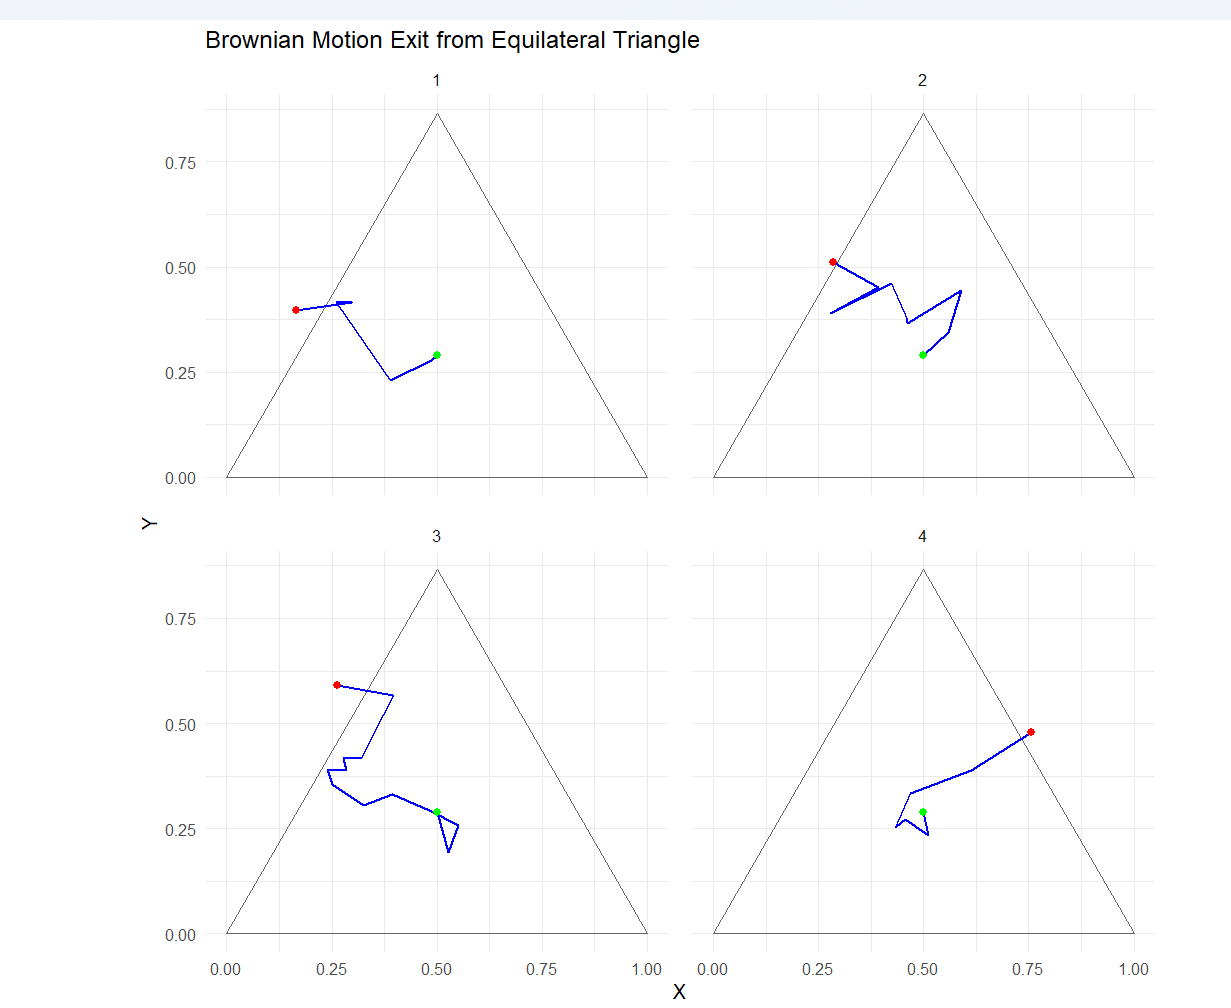
\includegraphics[width=0.7\columnwidth]{Screenshot 2025-07-05 141656.png}
    
\end{minipage}
%\hspace{1cm}
\vspace{1cm} %\\\vspace{-10cm}

%\hspace{1cm}
\begin{minipage}{\columnwidth}
    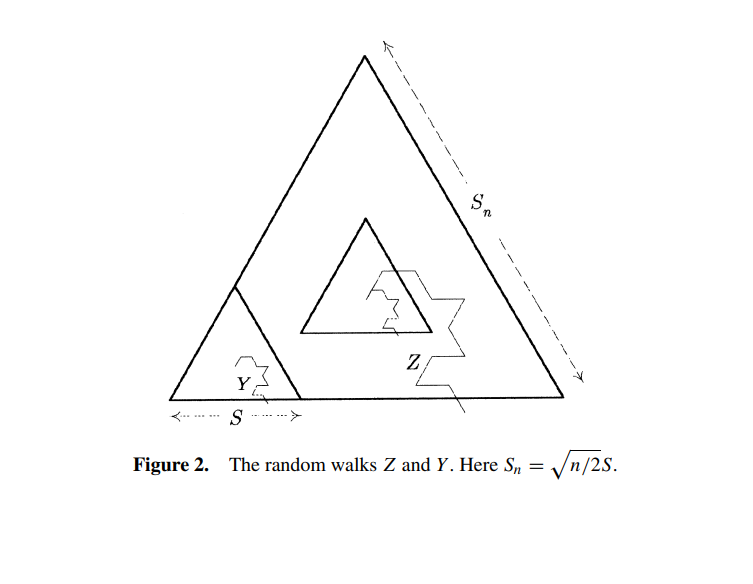
\includegraphics[width=0.6\columnwidth]{Screenshot 2025-07-03 132030.png}
\end{minipage}
%\hspace{1cm}

\section{Conclusion}
\begin{proposition}\cite{MR2023644}
The limit of the expected exit times from $\triangle_S$ of the approximating random walks $X^n$ is
\[
\frac{ \sqrt{3}\beta \left( \alpha - \frac{1}{\sqrt{3}}\beta \right) \left( S - \alpha - \frac{1}{\sqrt{3}}\beta \right) }{S}, \tag{14}
\]
where $(\alpha, \beta)$ is the starting point.
\end{proposition}
\begin{proof}
The set
\begin{align*}
\big\{(\alpha, \beta) \in \Delta_s :\ 
\sqrt{n/2}(\alpha, \beta)\ 
\text{ is a vertex of the triangular lattice for infinitely many } n\big\}
\end{align*}
is dense in $\Delta_s$. Define
\[
m =[\sqrt{n/2}S] + 1
\]
For $k = m - 1, m$,
\begin{align*}
a_k &= \frac{\sqrt{n/2} \cdot 2}{\sqrt{3}} \beta\\
b_k &= {\sqrt{n/2}}\left( \alpha - \frac{1}{\sqrt{3}} \beta \right)\\
c_k &= k - \sqrt{n/2} \left( \alpha + \frac{1}{\sqrt{3}} \beta \right)
\end{align*}
which follows that
\[
E\left( T(Z^n, \Delta_k) \right) = n \sqrt{3} \beta \left( \alpha - \frac{1}{\sqrt{3}} \beta \right)
\frac{k - \sqrt{n/2} \alpha - \sqrt{n/2} \left( \frac{1}{\sqrt{3}} \beta \right)}{k}
\]
From the previous lemma,
\[
\frac{1}{n} T\left(Z^n, \Delta_k\right) = T\left(X^n ,\Delta_{k/\sqrt{n/2}} \right)
\]
Thus we have
\[
\Delta_{(m-1)/\sqrt{n/2}} \subseteq \Delta_S \subseteq \Delta_{m/\sqrt{n/2}}
\]
Taking $n \to \infty$
\[
\lim_{n \to \infty} \mathbb{E}[T(X_n, \Delta_{S})] = 
\frac{ \sqrt{3}\beta\left(\alpha - \frac{1}{\sqrt{3}}\beta\right)\left(S - \alpha - \frac{1}{\sqrt{3}}\beta\right) }{S}
\]
\end{proof}
%

%----------------------------------------------------------------------------------------
%	REFERENCES
%----------------------------------------------------------------------------------------

%\bibliographystyle{IEEEtran}
%\bibliography{IEEEabrv,references}
\bibliographystyle{plain}
\bibliography{references}


%---------------------------------------------------
-------------------------------------
\end{multicols}

\end{mdframed}
\end{document}
